%% http://tp.lc.ehu.es/TAE/lectures/lecture4.pdf
% An anomaly is the breaking of a classical symmetry due to quantum corrections.
% More explicitly, we say we have an anomaly when Noether's theorem predicts a conserved current do to a symmetry in the classical action, which is shown to not be conserved when considering quantum corrections to the current.

From Noether's theorem, described in the following section, we know that any continuous symmetry of the Lagrangian $\mathcal{L}$ in a classical consideration will lead to a conserved current.
However, we know from the path integral formulation of \gls{qft} that for a system with fields $\phi $ and an external source $J$, it is the generating functional
\begin{equation}
  \label{eq:generating_functional}
  Z[J] \equiv
  \int \mathcal{D}\phi 
  \exp \left[
  i \left( S[\phi] + \int \mathrm{d}^4x J(x) \phi(x) \right)
  \right] 
\end{equation}
that must be invariant for a transformation to be a symmetry operation of the system.
Quantum corrections from the second quantization can lead to the symmetry group of the generating functional to be smaller than the symmetry group of the classical action, in which case we say there is an \emph{anomaly}.
In that case, the conserved current predicted by Noether's theorem is no longer protected by symmetry, as the operation is indeed not a symmetry of the system.
The terms breaking the classical conservation are called \emph{anomalies}.

It should also be noted that the terminology \emph{anomaly} and \emph{breaks the classical symmetry} are somewhat misleading;
there is no actual symmetry breaking -- in the quantum theory there is no symmetry to begin with, and a more fitting language to describe the situation is that there is an anomalous symmetry in the classical Lagrangian, which is not there in the ``real'' theory.
Thus, the situation must not be confused with spontaneous symmetry breaking, and there is no Goldstone boson present.

\section{Noether's theorem}
The following section is inspired by the derivation of~\textcite{kachelriessQuantumFieldsHubble2018}.

Noether's theorem is one of the most central results in theoretical quantum physics.
It relates continuous symmetries with conserved quantities, which for example explain fundamental principles such as conservation of momentum and conservation of energy.
Given a Lagrangian $\mathcal{L}(\phi_a, \partial_{\mu}\phi_a)$ dependent on the fields $\phi_a$, we will consider the variations $\delta\phi_a$ that leave the action, and thus equations of motion, invariant.
That is, the variations that are generators for some continuous symmetry of the system.
Firstly, we will restrict our consideration to the case where the Lagrangian itself is invariant
\begin{equation}
  0 = \delta \mathcal{L} =
  \frac{\delta \mathcal{L}}{\delta \phi_a} \delta\phi_a + \frac{\delta \mathcal{L}}{\delta\partial_{\mu}\phi_a} \delta\partial_{\mu}\phi_a.
\end{equation}
In the last term use that the variation and derivation may be exchanged, $[\delta\partial_{\mu}, \partial_{\delta}\delta] = 0$, and in the first term use the Lagrange equations
\begin{equation}
  \label{eq:lagrange_eq}
  \frac{\delta \mathcal{L}}{\delta\phi_a} = \delta_{\mu} \left( \frac{\delta \mathcal{L}}{\delta \partial_{\mu}\phi_a} \right).
\end{equation}
By the product rule it follows that
\begin{equation}
  \label{eq:noether-1}
  0 = \delta \mathcal{L} =
  \partial_{\mu}\left( \frac{\delta \mathcal{L}}{\delta\partial_{\mu}\phi_a} \right) \delta \phi_a
  + \frac{\delta \mathcal{L}}{\delta\partial_{\mu}\phi_a} \partial_{\mu}\delta \phi_a
  = \partial_{\mu} \left( \frac{\delta \mathcal{L}}{\delta\partial_{\mu}\phi_a} \delta\phi_a \right).
\end{equation}
Thus, we see that the quantity in the parenthesis after the last equality must be conserved.
We denote this quantity $j^{\mu}$ and call it a \emph{current}.

So far, we have the result that for any variation $\delta \phi_a$ that leave the Lagrangian invariant, there is a conserved current
\begin{equation}
  j^{\mu} = \frac{\delta \mathcal{L}}{\delta \partial_{\mu}\phi_a} \delta\phi_a, \quad \partial_{\mu}j^{\mu} = 0.
\end{equation}
There is, however, an even stronger formulation of Noether's theorem.
As the equations of motion are only dependent on the transformation being a symmetry transformation of the action, we realize that even a change in the Lagrangian of the form $\delta \mathcal{L} = \partial_{\mu}K^{\mu}$ will not change the equations of motion, as long as boundary terms of the integral over the Lagrangian may be dropped ($K\to  0, r \to \infty$).
Thus, altering the starting point in \cref{eq:noether-1} to $0 = \delta \mathcal{L} - \partial_{\mu}K^{\mu}$ we get Noether's theorem, theorem \ref{sec:noethers-theorem}.
\begin{theorem}[Noether's theorem]\label{sec:noethers-theorem}
  For any continuous transformation that leave the Lagrangian $\mathcal{L}$ invariant up to a total derivative $\partial _{\mu }K^{\mu }$, there must be an associated conserved current
  \begin{equation}
    \label{eq:noether_thm}
    j^{\mu} = \frac{\delta \mathcal{L}}{\delta \partial_{\mu} \phi_a} \delta \phi_a - K^{\mu}, \quad \partial_{\mu }j^{\mu } =0.
  \end{equation}
\end{theorem}


\section{The axial/chiral anomaly}
%% Note: look at https://www.damtp.cam.ac.uk/user/tong/gaugetheory/3anom.pdf
%% Note: could we include some of the discussion about
%%       Tr([a,adagger]) in https://www.damtp.cam.ac.uk/user/tong/gaugetheory/3anom.pdf
%%       This might be useful when later dealing with fingerprints approach.
We will first give a quick and somewhat superficial introduction to the axial anomaly,%
\footnote{Also known as the chiral anomaly.}
and why it matters in condensed matter physics.
That discussion will be based on the discussion given in~\textcite{wehlingDiracMaterials2014} and~\textcite[Ch.~3]{tongGaugeTheoryLecture}.
Then we will present a more thorough derivation of the anomaly, based on the derivation of~\textcite{zeeQuantumFieldTheory2010} and~\textcite{kachelriessQuantumFieldsHubble2018}.

In the massless case, the Dirac equation reduces to two Weyl equations, whose solutions are right- and left-moving fermions.
In 1+1 dimensions they have the energy dispersion
\[
  \epsilon  _{\pm} = \pm |p|,
\]
where the $\pm$ indicates positive and negative energy solutions.
Consider the case now in the Dirac sea picture.
The negative energy solutions, antiparticles in high energy physics and holes in condensed matter physics, are all filled, with the energy band going to $\pm \infty $ momentum.
The particles with energy $\epsilon  = +p$ are right-moving solutions, while $\epsilon  = -p$ represent left-moving solutions.
Note that in this language, an antiparticle with negative momentum, is right moving, and of course, a particle with positive momentum is right moving.
The situation is shown in the left pane of \cref{fig:chiral-dispersion}.
Introduce now an electric field \(E\).
This will cause the states to shift, according to $\dot{p} = e E$, with $e$ being the electric coupling, which is here taken to be the fundamental charge;
note that this shift does not discriminate against left- and right-movers, they are both shifted the same.
For a field $E > 0$ the right-movers are shifted towards higher energies and the left-movers are shifted towards lower energies, shown in the right pane of \cref{fig:chiral-dispersion}.
This also shifts the densities of left- and right-movers!
Denote by $n_+$ the right-movers and $n_-$ the left-movers.
The total density $n = n_+ + n_-$ is constant, however, the difference $n_+ - n_-$ is not conserved.
Identifying $J = n_+ + n_-$ as the vector current and $J_A = n_+  - n_{-}$ as the axial current, we see that the vector current is conserved, but the \emph{axial} current is not!
Notice how the origin of the anomaly in this context, is the infinite depth of the Dirac sea.

\begin{figure}[th]
  \centering
  % \resizebox{0.4\textwidth}{!}{
    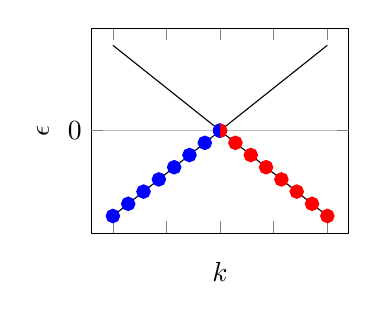
\begin{tikzpicture}
      \begin{axis}[
        cycle list shift=-2,
        width=0.4\textwidth,
        xlabel=\(k\),
        ylabel=\(\epsilon \),
        ytick=\empty,
        xticklabels={,,}, yticklabels={,,},
        extra y tick style = {grid = major },
        extra y tick labels = 0,
        extra y ticks = 0,
        legend columns = 3,
        legend entries = {Filled right movers, Filled left movers},
        legend style={/tikz/every even column/.append style={column sep=0.5cm}},
        legend to name=chiralLeg,
        domain=-4:4,
        ]
        \addplot [domain=-4:0, samples=8, mark=*, only marks, very thick, blue] {x};
        \addplot [domain=0:4, samples=8,  mark=*, only marks, very thick, red] {-x};
        \addplot[samples=2, mark=none] {x};
        \addplot[samples=2, mark=none] {-x};

        % \addplot[mark=halfcircle*, only marks, domain=0:0.5, mark repeat={2}, fill=blue, mark color=red, samples=2] {x};
        \coordinate (O) at (axis cs: 0,0);
      \end{axis}
        \begin{scope}
          \clip (O)+(-1,-1) rectangle ++(0,1);
          \fill[blue] (O) circle(0.092);
        \end{scope}
    \end{tikzpicture}
    % }
  % \resizebox{0.4\textwidth}{!}{
    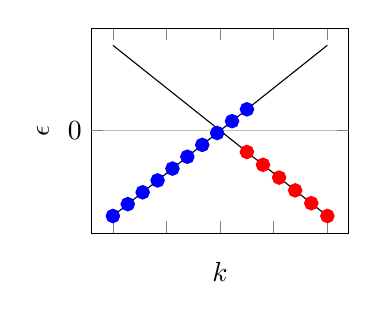
\begin{tikzpicture}
      \begin{axis}[
        cycle list shift=-2,
        width=0.4\textwidth,
        xlabel=\(k\),
        ylabel=\(\epsilon \),
        ytick=\empty,
        xticklabels={,,}, yticklabels={,,},
        extra y tick style = {grid = major },
        extra y tick labels = 0,
        extra y ticks = 0,
        domain=-4:4,
        ]
        \addplot[samples=2, mark=none] {x};
        \addplot[samples=2, mark=none] {-x};
        \addplot [domain=-4:1, samples=10, mark=*, only marks, very thick, blue] {x};
        \addplot [domain=1:4, samples=6, mark=*, only marks, very thick, red] {-x};
      \end{axis}
    \end{tikzpicture}\\

    % \tikzset{/tikz/external/export next=false}\ref{chiralLeg}  % Legend
    % \ref{chiralLeg}  % Legend
    \pgfplotslegendfromname{chiralLeg}
    %% NB!!! For the ref to work, you must manually!! call the jobnmme
    % }
    \caption{Dispersion of Weyl fermions, black showing unfilled states, blue filled right-movers, and red filled left-movers.
      \textbf{(Left)} No electric field applied, Fermi level at the crossing.
      \textbf{(Right)} Electric field in the positive direction applied, shifting the filled states.
      See main text for details.
    \label{fig:chiral-dispersion}}
\end{figure}

\begin{comment}
  % Taken  from wehling
  To put this in the context of condensed matter physics, we will consider the lowest Landau level in a 3D Weyl SM, with the energy $\epsilon = - s\hbar v_F \vec{k} \cdot \hat{B}$, where $s$ is the chirality of the Weyl point and $\hat{B}$ is the direction of the $\vec{B}$-field~\cite{arjonaFingerprintsConformalAnomaly2019}.
  Applying then an electric field $\vec{E}$ perpendicular to the magnetic field $\vec{B}$, all states will be shifted along the electric field according to $\hbar \vec\dot{k} = -e \vec{E}$, with the minus sign coming from the electron having negative charge.
  For the lowest level state, which is chiral, this means that electrons are either disappearing or appearing at the Weyl point.
  The charge is thus not locally conserved around the Weyl point, with the modified continuity equation
  \begin{equation}
    \frac{\partial n}{\partial t} + \nabla \cdot \vec{J} =
    \pm \frac{e^2}{4 \pi^2 \hbar^2 } \vec{E} \cdot \vec{B}.
  \end{equation}
  This non-conservation is an inherently quantum effect.
  Interestingly, this gives yet another explanation, in addition to the Chern conservation explanation, as to why Weyl points must always appear in pairs of opposite chirality, as overall the charge must of course be conserved.
  This gives rise to an interesting effect, which manifests itself in the materials transport properties.
  For a pair of opposite Weyl points separated in momentum space, the anomaly gives an imbalance between the two nodes
  \begin{equation}
    \frac{\partial (n_+ - n_-)}{\partial t} = \frac{e^2}{2 \pi^2 \hbar^2} \vec{E} \cdot \vec{B}.
  \end{equation}
  This charge imbalance, between the nodes separated in momentum space, can be relaxed only by a large momentum scattering, and thus the relaxation time is very long for systems with few impurities.
  This causes the conductivity along the direction of the magnetic field to increase~\cite{wehlingDiracMaterials2014}.
\end{comment}

The above argumentation gives an intuitive explanation and interpretation of the anomaly, but it is obviously not rigorous.
We here give a purely field theoretical derivation of the axial anomaly.
Consider a massless \gls{qft}
\( \mathcal{L} = \bar{\psi} i \gamma^{\mu}\partial_{\mu} \psi \),
which under the gauge transformation
\begin{equation}
  \psi \to  e^{i \theta + i\theta \gamma^5} \psi
\end{equation}
is invariant.
It can be shown that the associated conserved Noether currents are the vector current \( J^{\mu} = \bar{\psi} \gamma^{\mu} \psi \) and the axial current \( J_5^{\mu} = \bar{\psi} \gamma^{\mu} \gamma^5 \psi \)~\cite{zeeQuantumFieldTheory2010}.
In the following, we will show that the two currents \emph{cannot} be simultaneously conserved -- that is the chiral anomaly.
As is often the case, there are many ways to do this.
For example, one could show directly that the measure of the path integral is not invariant under a transformation.
We will, however, show it in a somewhat crude way, but where there are no complicated formal considerations, only brute force calculation which is hopefully more readily appreciated by those not familiar with the concept.
The calculation also has some historical importance, as the problem we will solve is exactly the same as the problem that led to the discovery of anomalies~\cite{adlerAxialVectorVertexSpinor1969,bellPCACPuzzleP01969}!%
\footnote{The anomaly was discovered independently by \textcite{adlerAxialVectorVertexSpinor1969} and \textcite{bellPCACPuzzleP01969} in 1969. See~\textcite{tongGaugeTheoryLecture} for a more in-depth historic commentary.}


We will calculate the triangle diagram
% \begin{figure}[h]
  % \centering
\begin{center}
  \tikzsetnextfilename{feynman-triangle}
  \nocite{ellisTikZFeynmanFeynmanDiagrams2017}
  %% NB! tikz-feynman must be compiled with lualatexx
  \feynmandiagram [vertical'=t2 to t3, small]{
    t1[label=left:\(\gamma ^{\lambda }\gamma ^5 \), left=3cm]  % 'longer' triangle
    -- [fermion, edge label=\(p\)] t2 [label=above:\(\gamma ^{\mu }\)]
    -- [fermion, edge label=\(p-k_1\)] t3 [label=below:\(\gamma ^{\nu }\)]
    --  [fermion, edge label=\(p-q\)] t1,
    t2 -- [photon] p1,
    t3 -- [photon] p2,
    p1 -- [opacity=0] p2, %% Helper line to make photons parallell
  };
\end{center}
% \end{figure}
and show that this leads to the conclusion that either the vector current or the axial current is non-conserved.
The amplitude of the diagram is
\begin{equation}
  \Braket{0|
    T J_5^{\lambda} J^{\mu} J^{\nu}|
  0},
\end{equation}
with the vector current $J^{\mu }= \bar{\psi} \gamma ^{\mu } \psi $ and the axial current $J_5^{\mu } = \bar{\psi} \gamma ^{\mu } \gamma ^5\psi $.
Written out explicitly in momentum space
\begin{equation}
  \label{eq:amplitude}
  \begin{split}
  &\mathcal{A}^{\lambda \mu \nu}(k_1, k_2) =
  (-1) i^3 \int \frac{\mathrm{d}^4p}{(2 \pi)^{4}}\\
  &\quad\times\operatorname{Tr}\left(
    \gamma^{\lambda}\gamma^5 \frac{1}{\slashed{p} - \slashed{q}}
    \gamma^{\nu} \frac{1}{\slashed{p} - \slashed{k}_{1}}
    \gamma ^{\mu} \frac{1}{\slashed{p}}
    % Next term %%%
    +
    \gamma ^{\lambda}\gamma^5 \frac{1}{\slashed{p} - \slashed{q}}
    \gamma ^{\mu } \frac{1}{\slashed{p} -\slashed{k}_{2}}
    \gamma ^{\nu } \frac{1}{\slashed{p}}
  \right),
  \end{split}
\end{equation}
where $q = k_1 + k_2$.
For the vector current to be conserved the requirement $k_{1\mu }\mathcal{A} ^{\lambda \mu \nu } = k_{2\nu }\Delta ^{\lambda \mu \nu } = 0$ must hold.
For the axial current to be conserved, the requirement is $q_{\lambda }\mathcal{A}^{\lambda \mu \nu } = 0$~\cite{zeeQuantumFieldTheory2010}.
% \todo{show or cite the requirements. I think maybe it is quite simple to see from the wick contractions}

One must be careful when carrying out this calculation, as is also stressed in many textbooks dealing with this issue, for example~\cite{kachelriessQuantumFieldsHubble2018} and~\cite{zeeQuantumFieldTheory2010}.
Consider the criterion for the vector current to be conserved
\begin{equation}
  \label{eq:criterion-conserved}
  k_{1\mu } \mathcal{A} ^{\lambda \mu \nu } (k_1, k_2) =
  i\! \int\! \frac{\mathrm{d}^4p}{ (2\pi)^{4}}
  \operatorname{Tr}\left(
    \gamma ^{\lambda } \gamma ^5 \frac{1}{\slashed{p} - \slashed{q}} \gamma ^{\nu}
    \frac{1}{\slashed{p} - \slashed{k}_{1}}
    -
    \gamma ^{\lambda }\gamma ^5 \frac{1}{\slashed{p} -\slashed{k}_{2}} \gamma ^{\nu }\frac{1}{\slashed{p}}
  \right)
  = 0.
\end{equation}
When calculating the integral it might be tempting to simply perform a change of variables, rendering the two terms equal and thus concluding that the criterion is met.
However, we must notice that the integrand goes like $1 / p^2$ while the boundary surface of a 3-sphere is proportional to $p^3$.
The boundary terms do therefore not vanish, and there is an extra term associated with performing such a change of variables.

Consider that we want to integrate over the function $f$
\begin{equation}
  \int \mathrm{d}^dp f(p).
\end{equation}
If we perform the change of variables $p \to p+a$, one could in theory get an extra contribution from boundary terms, which we will now find.
We will calculate
\begin{equation}
  \int \mathrm{d}^dp \left[ f(p+a) - f(p) \right],
\end{equation}
where we in the first term has ``naively'' performed a change of variables, without considering the boundary terms.
Thus, the result of this integral is indeed the boundary terms.
Firstly, we will perform a Wick rotation into Euclidean space
\todo{some note about why this is allowd, i.e. that there exists some Feynamn parametrization for the}%
\begin{equation}
  \int \mathrm{d}^d_Ep \left[ f(p+a) - f(p) \right]
  = \int \mathrm{d}_E^d p \left[ a^{\mu }\partial_{\mu} f(p) + \dots \right].
\end{equation}
Ignoring the higher order terms, the RHS may be rewritten as a surface integral by Gauss's theorem.
Taking the average over the surface integral, and denoting by $S_d(r)$ the surface of a d-sphere with radius r, we write the integral as
\begin{equation}
  \lim_{P\to \infty } a^{\mu } \left( \frac{P_{\mu }}{P} \right) f(P) S_{d-1}(P).
\end{equation}
Rotating back to Minkowski space we gain an additional i, with
\begin{equation}
  \label{eq:shift-trickery}
  \int \mathrm{d}^{d}p \left[ f(p+a) - f(p) \right]
  = \lim_{P\to \infty } ia^{\mu } \left( \frac{P_{\mu }}{P} \right) f(P) S_{d-1}(P).
\end{equation}

We will now perform such a shift of variables in the second term of the trace in \cref{eq:criterion-conserved}, as we notice that shifting $p \to p-k_1$ makes the two terms cancel, leaving only the boundary term.
Let
\begin{equation}
  \label{eq:trace-trickery}
  f(p) = \operatorname{Tr}\left(
  \gamma ^{\lambda }\gamma ^5 \frac{1}{\slashed{p} - \slashed{k}_2} \gamma ^{\nu } \frac{1}{\slashed{p}}
  \right)
  = \frac{\operatorname{Tr}\left(
  \gamma ^5 (\slashed{p}-\slashed{k}_2) \gamma ^{\nu }\slashed{p}\gamma ^{\lambda }
\right)}{
(p-k_2)^2 p^2}
= \frac{{4 i \epsilon ^{\tau \nu \sigma \lambda } k_{2\tau }P_{\sigma }}}{(p-k_2) p^2}.
\end{equation}
Here we used in the first equality the property $1 /\slashed{a} = \slashed{a} /a^2$ twice, and the cyclic permutation invariance of the trace, $\operatorname{Tr}(ABC) = \operatorname{Tr}(BCA)$.
In the second equality, we first wrote the Feynman slash operator by its definition $\slashed{a}=\gamma ^{\mu }a_{\mu }$, and then used the property
\begin{equation}
  \label{eq:trace-gamma}
  \operatorname{Tr}(\gamma ^5\gamma ^{\tau }\gamma ^{\nu }\gamma ^{\sigma }g^{\lambda }) = -4i\epsilon ^{\tau \nu \sigma \lambda },
\end{equation}
where $\epsilon $ is the totally antisymmetric tensor.
The trace can be split into two terms, where the first vanishes as it is proportional to $\epsilon ^{\tau \nu \sigma \lambda }p_{\tau }p_{\sigma }$, and one is left with the expression in \cref{eq:trace-trickery}.
Thus, \cref{eq:criterion-conserved} becomes
\begin{equation}
  \label{eq:criterion-conserved-simp}
  k_{1\mu } \mathcal{A}^{\lambda \mu \nu } =
  \frac{i}{(2\pi)^{4}} \lim_{P\to \infty } i(-k_1)^{\mu } \frac{P_{\mu }}{P}
  \frac{{4 i \epsilon ^{\tau \nu \sigma \lambda } k_{2\tau } P_{\sigma }}}{P^{4}} 2\pi^2 P^3
  = \frac{i}{8\pi^2} \epsilon ^{\lambda \nu \tau \sigma } k_{1\tau }k_{2\sigma }.
\end{equation}

Consider now, however, what happens if we shift $p\to p+k_2$ in the first term of \cref{eq:criterion-conserved} instead.
Surely, if our answer above is correct, any arbitrary shift must yield the same answer.
Similarly to before, let
\begin{equation}
  \begin{split}
    f(p) &= \Tr\left(\gamma^{\lambda }\gamma^5 \frac{1}{\slashed{p} - \slashed{q}} \gamma^{\nu } \frac{1}{\slashed{p} - \slashed{k}_{1}} \right)
         = \frac{\Tr \left( \gamma ^5 (\slashed{p}-\slashed{q}) \gamma ^{\nu } (\slashed{p}-\slashed{k}_1)\gamma ^{\lambda } \right)}{
           (p-q)^2(p-k_1)^2
           }\\
         &=
           \frac{-4i\epsilon ^{\tau \nu \sigma \lambda } k_{2\tau } (k_{1\sigma } - p_{\sigma })}{
           (p-q)^2(p-k_1)^2
           },
  \end{split}
\end{equation}
where we as above removed all terms symmetric under $\sigma \leftrightarrow \tau$.
Now, \cref{eq:criterion-conserved} becomes
\begin{equation}
  k_{1\mu } \mathcal{A}^{\lambda \mu \nu } =
  \frac{i}{(2\pi)^4} \lim_{P \to \infty } ik_2^{\mu } \frac{P_{\mu }}{P}
  \frac{{-4i\epsilon ^{\tau \nu \sigma \lambda } k_{2\tau } (k_{1\sigma }-p_{\sigma })}}{P^{4}}
  2\pi^2P^3
  = \frac{ i \epsilon ^{\lambda \nu \tau \sigma } }{8\pi^2}  k_{2\tau }k_{2\sigma }.
\end{equation}
\todo{Check there is not misssing a -1 in last espression}%
Where we used that the only term contributing is the $p_{\sigma }$, as the term with $k_{1\sigma }$ goes like $P^{-1}$.
Our results differ depending on the non-physical shift of variables!
As is shown by several textbooks, see~\cite{zeeQuantumFieldTheory2010,kachelriessQuantumFieldsHubble2018}, this comes from the fact that the integral we started with is in fact linearly divergent -- its value is not well-defined.
What we will have to do, is consider an arbitrary shift $a$ in the integration variable of the amplitude \cref{eq:amplitude}, which we will show changes the amplitude by a quantity dependent on $a$.
To cancel this, a counter term must be inserted;
however, as we will see, this counter term can only make either the axial current or the vector current conserved!
Consider now a shift in the integration variable $p \to p - a$ in the amplitude \cref{eq:amplitude}, where we denote the amplitude with shifted integration variable
\begin{equation}
  \label{eq:amplitude-shift}
  \begin{split}
    &\mathcal{A}^{\lambda \mu \nu}(a, k_1, k_2)\\
    &\quad=
  (-1) i^3 \int \frac{\mathrm{d}^4p}{(2\pi)^{4}}
  \begin{multlined}[t]
    \Tr \left(
      \gamma ^{\lambda } \gamma ^5 \frac{1}{\slashed{p} - \slashed{a} - \slashed{q}} \gamma ^{\nu } \frac{1}{\slashed{p} - \slashed{a}- \slashed{k}_{1}} \gamma ^{\mu } \frac{1}{\slashed{p} - \slashed{a}} \right.\\
   \quad +
    \left. \gamma ^{\lambda }\gamma ^5 \frac{1}{\slashed{p} - \slashed{a}- \slashed{q}} \gamma ^{\mu } \frac{1}{\slashed{p} - \slashed{a} - \slashed{k}_2} \gamma ^{\nu } \frac{1}{\slashed{p} - \slashed{a}}
    \right).
  \end{multlined}
  \end{split}
\end{equation}

From \cref{eq:shift-trickery} we already have a formula for the difference
\begin{equation}
  \label{eq:amplitude-difference}
  \mathcal{A}^{\lambda \mu \nu } (a, k_1, k_2) - \mathcal{A}^{\lambda \mu \nu }(k_1, k_2),
\end{equation}
by choosing
\[
  f(p) = \frac{i}{(2\pi)^{4}} \Tr \left( \gamma ^{\lambda }\gamma ^5 \frac{1}{\slashed{p} - \slashed{q}} \gamma ^{\nu } \frac{1}{\slashed{p} - \slashed{k}_{1}} \gamma ^{\mu } \frac{1}{\slashed{p} } \right). 
\]
Ignore for now the prefactor, and note that in the limit
\begin{equation}
  \begin{split}
    \lim_{p\to \infty } f(p) &=
    \frac{\Tr(\gamma ^{\lambda }\gamma ^5 \slashed{p} \gamma ^{\nu } \slashed{p}\gamma ^{\mu }\slashed{p})}{p^6}\\
    &= \frac{2 \Tr(\gamma ^{\lambda }\gamma ^5 \slashed{p}\gamma ^\nu \slashed{p}) - p^2\Tr(\gamma ^{\lambda }\gamma ^5 \slashed{p} \gamma ^{\nu }\gamma ^{\mu })}{p^6}\\
    &= \frac{{4i p_{\sigma }\epsilon ^{\sigma \nu \mu \lambda }}}{p^{4}}.
  \end{split}
\end{equation}
In the second equality we used the anti-commutation relation of gamma matrices in $\slashed{p} \gamma ^{\mu } = 2p^{\mu } - \gamma ^{\mu } \slashed{p}$ and $\slashed{a}^2 = a^2$.
In the last equality, we used again \cref{eq:trace-gamma}, and the vanishing of all terms symmetric under interchanging indices when contracted with the fully antisymmetric tensor.
We now find the amplitude difference \eqref{eq:amplitude-difference}.
Firstly, we simplify the  expression slightly as
\begin{equation}
  \Delta \mathcal{A}^{\lambda \mu \nu }(a, k_1, k_2) \equiv \int \mathrm{d}^4p f(p-a) - f(p) +  \{(k_1,\mu ) \leftrightarrow (k_2, \nu )\},
\end{equation}
where the last term indicates to repeat the preceding expression with interchange of $k_1 \leftrightarrow  k_2$ and $\mu \leftrightarrow \nu$.
Thus, by \cref{eq:shift-trickery},
\begin{equation}
  \label{eq:amplitude-difference-explicit}
  \begin{split}
  \Delta \mathcal{A}^{\lambda \mu \nu}(a, k_1, k_2) &=
%  \lim_{p\to \infty } i  a^{\mu } \left( \frac{p_{\mu }}{p} \right) f(p) 2\pi^2p^3
    \lim_{p\to \infty } i  a^{\mu } \left( \frac{p_{\mu }}{p} \right)
  \frac{i}{(2\pi)^{4}} \frac{{4ip_{\sigma }\epsilon ^{\sigma \nu \mu \lambda }}}{p^{4}}
  2\pi^2p^3\\
  &\quad + \{(k_1,\mu ) \leftrightarrow (k_2, \nu )\}\\
  &= \lim_{p\to \infty } \frac{{-ia^{\mu }}}{2\pi^2} \frac{{p_{\mu }p_{\sigma }}}{p^2} \epsilon ^{\sigma \nu \mu \lambda } +  \{(k_1,\mu ) \leftrightarrow (k_2, \nu )\}\\
  &= - \frac{ia_{\sigma }}{8 \pi^2}\epsilon ^{\sigma \nu \mu \lambda } +  \{(k_1,\mu ) \leftrightarrow (k_2, \nu )\}.
  \end{split}
\end{equation}
\todo{Figure out if there is missing an overall minus sign}%

Now is the time to take a break from the calculations and consider in some detail what this result means, before we will finally carry out the derivation to its end and show the anomaly.
A priori $\mathcal{A}^{\lambda \mu \nu }(a, k_1, k_2)$ should be just as valid as $\mathcal{A}^{\lambda \mu \nu }(k_1,  k_2)$, i.e. setting $a=0$.
In fact, that formulation is quite the misnomer, as $a=0$ is no less arbitrary than any $a\neq 0$ in this setting;
% $p$ is simply a name we have denoted the momentum transfer in our diagram.
$p$ is simply a name by which we denote the moment transfer in our diagram.
\emph{However}, using \cref{eq:amplitude-difference-explicit}, leading to
\begin{equation}
  \label{eq:19}
  \begin{split}
  &k_{1\mu } \mathcal{A}^{\lambda \mu \nu }(a, k_1, k_2) - k_{1\mu }\mathcal{A}^{\lambda \mu \nu }(a=0, k_1, k_2) \\
 &\quad = -\frac{i}{8\pi^2} \left[
  \epsilon ^{\sigma \nu \mu \lambda } a_{\sigma } +  \{(k_1,\mu ) \leftrightarrow (k_2, \nu )\} \right] k_{1\mu }, 
  \end{split}
\end{equation}
we see that the criterion for vector current conservation, \cref{eq:criterion-conserved}, may or may not be met depending on our choice of $a$!
\todo{Should this be related to counter terms as Kachelriess does? What does it really mean that we have to choose some shift}%
Owning to a trick from~\textcite{zeeQuantumFieldTheory2010}, we will show that the resolve of this is to chose one particular $a$, and the choice will be that $a$ which preserves the consistency of our theory.
Now, this may indeed seem both strange and ad-hoc, how can we justify \emph{choosing} some parameter to get the result we want?
This is, in fact, common in \gls{qft}.
Recall that both the UV-cutoff and dimensional regularization schemes introduce a parameter, which must be determined ``outside'' of our theory.

Let $a=\alpha (k_1+k_2) + \beta (k_1-k_2)$.
This is allowed as $k_1, k_2$ are independent, and the only parameters of our equations.
The $\alpha$ term is obviously symmetric under interchange of $k_1, k_2$, while the $\beta$ term is antisymmetric.
Thus, we see that in \cref{eq:19} only the $\beta $ part survives when adding the pair with interchanged indices and momenta.
Thus,
\begin{equation}
  \begin{split}
  k_{1\mu }\mathcal{A}^{\lambda \mu \nu }(a, k_1, k_2) &=
                                                         -\frac{i}{4\pi^2} \epsilon ^{\sigma \nu \mu \lambda } \beta (k_{1\sigma } - k_{2\sigma })k_{1\mu } + k_{1\mu }\mathcal{A}^{\lambda \mu \nu }(k_1, k_2)\\
                                                       &= \frac{i}{8\pi^2} \left(
                                                         \epsilon ^{\lambda \nu \tau \sigma }k_{1\tau }k_{2\sigma } - 2 \epsilon ^{\sigma \nu \mu \lambda } \beta (k_{1\sigma } - k_{2\sigma })k_{1\mu }\right)\\
  &= \frac{i}{8\pi^2} \epsilon ^{\lambda \nu \tau \sigma } k_{1\tau }k_{2\sigma } (1+ 2\beta ).
  \end{split}
\end{equation}
Here we inserted our previous result for $k_{1\mu }\mathcal{A}^{\lambda \mu \nu }$ given in \cref{eq:criterion-conserved-simp}.
In the last equality, we used that $k_{1\sigma }k_{1\mu }$ vanishes when contracted with the Levi Cevita symbol, and relabeled the dummy indices.
It is now apparent that choosing $\beta = -1 / 2$ makes the criterion for conservation of vector current hold!

By choosing the shift appropriately, the vector current is preserved.
However, it does come at a price.
The requirement for the axial current to be conserved, as mentioned earlier, is
\[
  q_{\lambda } \mathcal{A}^{\lambda  \mu  \nu } = 0.
\]
This amplitude is in fact also set by the parameter $\beta $, as also here $\alpha $ drops out;
we have no free parameter to tune after fixing $\beta $.
With the choice $\beta  = -1 / 2$, required to conserve the vector current, the axial current will not be conserved!
This is the chiral anomaly.

We could have, of course, instead chosen $\beta $ such that the axial current is conserved, at the expense of the conservation of the vector current.
However, as~\textcite{zeeQuantumFieldTheory2010} describes, this would have catastrophic consequences, rendering the entire theory useless.
A non-conserved vector current would make the fermion number not conserved, clearly non-acceptable.
We therefore chose to sacrifice the axial current instead of the vector current.


\section{The conformal/scale anomaly}
Consider massless \gls{qed}
\begin{equation}
  \mathcal{L} = -\frac{1}{4} F^{\mu\nu}F_{\mu\nu} + i \bar{\psi} \slashed{D} \psi,
\end{equation}
with $\psi$ the Dirac field, $\bar{\psi} = \psi^{\dagger}\gamma^0$, $\slashed{D} = \gamma^{\mu} D_{\mu}$, $D$ the covariant derivative $D_{\mu} = \partial_{\mu}-ieA_{\mu}$, $\gamma^{\mu}$ the Dirac matrices.
$A_{\mu}$ is the electromagnetic potential, $F_{\mu \nu} = \partial _{\mu }A_{\nu } - \partial _{\nu } A_{\mu }$ the electromagnetic field, and $e$ is the coupling, here the fundamental charge.
The theory is classically scale-invariant.
That is, under the transformation
\begin{equation}
  x \to \lambda^{-1} x, \quad A_{\mu} \to  \lambda A_{\mu}, \quad \psi \to  \lambda^{\frac{3}{2}}\psi,
\end{equation}
the Lagrangian transforms as
\begin{equation}
  \mathcal{L} \to \lambda^4 \mathcal{L},
\end{equation}
which is canceled by the transformation of measure $\mathrm{d}^4 x \to \mathrm{d}^4x \lambda ^{-4}$ in the action.
As the action is invariant, thus so are the equations of motion.

By Noether's theorem, there must be some conserved current corresponding to this symmetry transformation, which we will now show is the dilation current $j_D^{\mu } = T^{\mu \nu } x_{\nu }$, where \( T^{\mu \nu} \) is the energy-momentum tensor.
Consider a conformal transformation of the type $g_{\mu \nu } = e^{2\tau } \eta _{\mu \nu }$, also known as a Weyl transformation of the metric.
The variation of the metric is obviously $\delta g_{\mu \nu } = 2 \tau \eta _{\mu \nu }$.
Recall also that the energy-momentum tensor is defined as the response of the action to a variation of the metric%
\footnote{This defines the \emph{dynamical} energy-momentum tensor. See \cref{sec:commen-T} for more details.}
\begin{equation}
  T_{\mu \nu } = \frac{2}{\sqrt{|g|}} \frac{{\delta S}}{\delta  g^{\mu \nu }},
\end{equation}
where $g$ is the determinant of the metric.
Now, using this we see that
\begin{equation}
  \label{eq:diff-action}
  \begin{split}
    \delta  S &= \int \mathrm{d}^4x \frac{\delta S}{\delta g^{\mu \nu }} \delta g^{\mu \nu }\\
    &= \int \mathrm{d}^4x \frac{\sqrt{|g|}}{2 } T_{\mu \nu } \delta g^{\mu \nu }\\
    &= \int \mathrm{d}^4x T_{\mu \nu } \sqrt{|g|} \tau (x) \eta ^{\mu \nu }(x)\\
    &= \int \mathrm{d}^4x \sqrt{|g|} \tau (x) T^{\mu }_{\mu }.
  \end{split}
\end{equation}
As the scaling is a symmetry operation, \cref{eq:diff-action} must be zero.
As the scaling factor $\tau $ is an arbitrary function, we conclude that the trace $T^{\mu }_{\mu }$ must vanish.
The vanishing trace ensures the conservation of the dilation current as
\begin{align}
  \label{eq:dilation-diff}
  \partial _{\mu } J_D^{\mu } &= T^{\mu \nu }\partial_{\mu } x_\nu +
                                (\overbrace{ \partial _{\mu }T^{\mu \nu } }^{0}) x_{\nu }\\
  \nonumber &= T^{\mu \nu }\delta _{\mu \nu } = T^{\mu }_{\mu },
\end{align}
where we used the property of the energy-momentum tensor that $\partial _{\mu }T^{\mu \nu } = 0$.
As the trace is zero, the dilation current is conserved in the classical picture.

However, this symmetry does not hold when quantum corrections are taken into account.
Loop effects give non-vanishing contributions to the trace, and by \cref{eq:dilation-diff} this makes the dilation current non-conserved.
Due to this, the conformal anomaly is also often referred to as the trace anomaly.
% Firstly, an intuitive and quick explanation for why the loop effect breaks the symmetry will be given, and then a more lengthy calculation showing this explicitly.
Recall that when calculating the propagators of the \gls{qed} theory, we end up with infinities.
These, we regularize and renormalize, for example with dimensional regularization or UV-cutoff.
In any case, this introduces some dimensionful scale, $\mu $, the renormalization scale and the cutoff energy respectively for the regulators mentioned.
This scale dependence is encoded in the beta function of the theory, encoding the dependence of the coupling $e$ on the scale,
\begin{equation}
  \beta (e) = \frac{\partial e}{\partial \log \mu };
\end{equation}
if the beta function does not vanish, our theory now has a scale dependence, rendering our theory no longer scale-invariant!

% Consider having a derivation of the conformal anomaly here.

When taking into account the loop effects, the trace of the energy-momentum tensor is~\cite{kachelriessQuantumFieldsHubble2018}
\begin{equation}
  T_{\mu }^{\mu } = \frac{\beta (e)}{2 e} F_{\mu \nu }F^{\mu \nu },
\end{equation}
where $\beta (e)$ is the beta function of the theory.
This beta function makes the anomaly not exact in one loop, as opposed to the axial anomaly.
In one loop, the massless fermion beta function is~\cite{chernodubAnomalousTransportDue2016}
\begin{equation}
  \label{eq:beta-function}
  \beta ^{(1)} = \frac{e^3}{12 \pi^2}.
\end{equation}

\begin{comment}
  Relating the perturbation $\tau $ to the gravitational potential $\phi $.
  In the Newtonian limit of general relativity, corresponding to $v /c \to 0$, the metric reduces to~\cite{kachelriessQuantumFieldsHubble2018}
  \begin{equation}
    \mathrm{d}s^2 = \left( 1 + 2\Phi  \right) \mathrm{d}t^2 - \left( 1 - 2 \Phi  \right) \left( \mathrm{d}x^2 + \mathrm{d}y^2 + \mathrm{d}z^2 \right),
  \end{equation}
  with $\Phi $ being the well-known Newtonian gravitational potential, coupling to the mass as
  \begin{equation}
    \mathcal{L}_{\text{gravity}} = -\rho \Phi.
  \end{equation}
  \todo{This above is taken simply from my memory. Verify}
  Thus, we see that, remembering the definition of the line element $ds = g_{\mu \nu } \mathrm{d}x^{\mu } \mathrm{d}x^{\nu }$,
  \begin{equation}
    g_{00} = 1 + 2\Phi .
  \end{equation}

  Thus, for a conformal transformation of the metric
  \[
    g_{\mu \nu } = e^{2\tau }\eta _{\mu \nu }, \quad \tau << 1,
  \]
  we identify the Newtonian gravitational potential as $\Phi = 2\tau $
\end{comment}

\begin{comment}
  \section{Notes for the section}
  %% Notes for this section:
  In order to better understand this ... introduce \gls{qft}, Path Integral, Chiral Anomaly
  The renormalization introduces a scale-invariance breaking quantity $\mu$.

  Anomalies must not be confused with spontaneous symmetry breaking, where sym of state is lower than sym of hamiltonian.

  These anomalous currents may give novel transport laws not present in the classical theory.

  There is some word for magnetically reduced/increased conductivity I believe. Magneto-somethingsomething

  The \emph{conformal} scale transformation $g \to g' = e^{2\omega} g$ because lengths are rescaled by a constant factor, while angles are conserved (Kachelriess (17.1))


  Is it not insane that adding the fictitious gravitational potential as we do in Luttinger's approach, can here be treated as an actual metric perturbation!! ???
\end{comment}
